\documentclass{article}
\usepackage{amsmath,amsthm,amssymb,amsfonts}
\usepackage{setspace,enumitem}
\usepackage{graphicx}
\usepackage{hyperref}
\usepackage{natbib}
\usepackage{afterpage}
\usepackage{xcolor}
\usepackage{etoolbox}
\usepackage{booktabs}
\usepackage{pdfpages}
\usepackage{multicol}
\usepackage{soul}
\usepackage{geometry}
\usepackage{accents}
\usepackage{accents}
\hypersetup{
	colorlinks,
	linkcolor={blue!90!black},
	citecolor={red!90!black},
	urlcolor={blue!90!black}
}
\usepackage{setspace}

\newtheorem{theorem}{Theorem}
\newtheorem{assumption}{Assumption}
\newtheorem{definition}{Definition}
\newtheorem{proposition}{Proposition}
\newtheorem{lemma}{Lemma}
\newcommand{\R}{\mathbb{R}}
\newcommand{\N}{\mathbb{N}}
\newcommand{\Lfn}{\mathcal{L}}
\newcommand{\Int}{\text{Int}}
\newcommand{\ubar}[1]{\underaccent{\bar}{#1}}
\newcommand{\xbf}{\mathbf{x}}
\newcommand{\Abf}{\mathbf{A}}
\newcommand{\Bbf}{\mathbf{B}}
\newcommand{\Gbf}{\mathbf{G}}
\newcommand{\bbf}{\mathbf{b}}

\setlength\parindent{0pt}

\title{ECON 736A: Problem Set 2}
\author{Alex von Hafften}
\date{\today}

\begin{document}

\maketitle

\textbf{Prompt:} Write a \textbf{simple} model of something.

\bigskip

\textbf{Idea:} A simple three period model of firm bankruptcy and reorganziation with debt dilution from long and short-term debt.

\bigskip

\textbf{General Timing:}

\begin{itemize}
\item Period 0
\begin{itemize}
\item Firm is born with funds $I$
\item Firm sells $b_0$ discount bonds at price $q_0$ to representative risk-neutral ``long-term" investor who can also buy risk-free discount bonds with price $\tilde q$
\end{itemize}
\item Period 1
\begin{itemize}
\item First productivity shock $\varepsilon_1 \sim F$ realized
\item Firm sells $b_1$ discount bonds at price $q_1$ to representative risk-neutral ``short-term" investor who can also buy risk-free discount bonds with price $\tilde q$
\item Firm buys capital $k \equiv I + q_0 b_0 + q_1 b_1$ and has outstanding debt $b \equiv b_0 + b_1$
\end{itemize}
\item Period 2
\begin{itemize}
\item Second productivity shock $\varepsilon_2 \sim G$ realized
\item Firm chooses to produce or default or reorganize
\begin{itemize}
\item If firm produces, firm payoff is $f(\varepsilon_1, \varepsilon_2, k) - b$, long-term investor payoff is $b_0$, and long-term investor payoff is $b_1$
\item If firm defaults, firm payoff is 0, long-term investor's payoff is $m_0(b_0, b_1) (1-\xi) f(\varepsilon_1, \varepsilon_2, k)$, short-term investor's payoff is $m_1(b_0, b_1) (1-\xi) f(\varepsilon_1, \varepsilon_2, k)$ where $\xi \in [0,1]$, $m_0(b_0,b_1) + m_1(b_0, b_1) \le 1$, $m_0(b_0,b_1) \ge 0$, and $m_1(b_0, b_1) \ge 0$ for all $b_0, b_1$
\item If firm chooses to reorganize, firm produces and firm and lenders Nash bargain over $f(\varepsilon_1, \varepsilon_2, k)$.
\end{itemize}
\end{itemize}
\end{itemize}

\pagebreak

\section*{With binary productivity shocks}

\subsection*{Assumptions:}

\begin{itemize}
\item In period 2, firm can only choose to produce or default (no reorganizing)
\item Recovery value is zero: $\xi = 1$
\item $\varepsilon_1$ and $\varepsilon_2$ are iid Bernoulli random variables that take $R > 1$ with probability $p$ and $1$ with probability $1 - p$
\item One type of debt: $b_1 = 0$
\item Production function $f(\varepsilon_1,\varepsilon_2, k) = \varepsilon_1\varepsilon_2k^\alpha$ where $\alpha \in (0,1)$
\end{itemize}

With these assumptions, problem is equivalent to two period model with one productivity shock 

$$
\tilde \varepsilon = 
\begin{cases} 
R^2, & \text{with probability } p^2\\
R, & \text{with probability } 2p(1-p)\\
1, & \text{with probability } (1-p)^2
\end{cases}
$$

\smallskip

\subsection*{Timing with simplifying assumptions:}

\begin{itemize}
\item Period 0
\begin{itemize}
\item Firm is born with funds $I$
\item Firm sells $b$ discount bonds at price $q$ to representative risk-neutral investor who can also buy risk-free discount bonds with price $\tilde q$
\item Firm buys capital $k \equiv I + q b$ 
\end{itemize}
\item Period 1
\begin{itemize}
\item Productivity shock $\tilde \varepsilon$ realized
\item Firm chooses to produce or default
\begin{itemize}
\item If firm produces, firm payoff is $\tilde \varepsilon k^\alpha - b$, and investor payoff is $b$
\item If firm defaults, firm payoff is 0, investor's payoff is 0
\end{itemize}
\end{itemize}
\end{itemize}

\subsection*{Solution}

\begin{itemize}

\item In period 1, firm produces iff $\tilde \varepsilon k^\alpha - b \ge 0 \implies \tilde \varepsilon \ge \frac{b}{k^\alpha}$. Notice that this threshold is increasing in $b$ and decreasing in $k$. That is if the firm has more debt (or less capital), it defaults for a larger set of productivity shocks.

\item Thus, the firm's profit is

\begin{align*}
\pi(\tilde \varepsilon, k, b) 
=
\begin{cases} 
\tilde \varepsilon k^\alpha - b, & \text{if }  \frac{b}{k^\alpha} \le \tilde\varepsilon \le 1 \\ 
0, & \text{if } 0 \le \tilde\varepsilon < \frac{b}{k^\alpha} 
\end{cases}
\end{align*}

\item Four cases for intermediate productivity shock: (1) firm always defaults, (2) firm only produces for $\tilde \varepsilon = R^2$, (3) firm only produces for $\tilde \varepsilon = R^2$ and $\tilde \varepsilon = R$ and (4) firm always produces. Let $\pi^{(j)}$ denote profit in case $j$.

\subsubsection*{Case 1: Firm always defaults}

\item Then, profit is zero for firm, $\pi^{(1)} = 0$. And $b=0$. Would be better not default for at least $\varepsilon = R^2$ with expected profit at least $p^2 R^2 I^\alpha > 0$ $\Rightarrow \Leftarrow$. The firm never always defaults.

\subsubsection*{Case 2: Firm only produces for $\tilde\varepsilon = R^2$}

\item Expected profit for $(k,b)$ is

$$
\pi(k, b) = p^2 (R^2 k^\alpha - b)
$$

\item Taking $q$ as given, the firm chooses $k$ and $b$ to maximize expected profit

\begin{align*}
\max_{k,b} & p^2 R^2 k^\alpha  - p^2 b\\
\text{s.t. } k &= I + qb\\
\Lfn &= p^2 R^2 k^\alpha  - p^2 b + \lambda(I + qb - k)
\end{align*}

\item FOCs

\begin{align*}
\alpha p^2 R^2 k^{\alpha-1} &= \lambda\\
p^2 &= q\lambda\\
\implies
q\alpha p^2 R^2 k^{\alpha-1} &= p^2\\
\implies
k &= q^{\frac{1}{1-\alpha}}\alpha^{\frac{1}{1-\alpha}}  R^{\frac{2}{1-\alpha}} 
\end{align*}

Higher $q$ (or lower interest rate) means more capital. Makes sense.

\item Debt demand is

\begin{align*}
b 
&= \frac{1}{q}(k  - I) \\
&= \frac{1}{q}[q^{\frac{1}{1-\alpha}}\alpha^{\frac{1}{1-\alpha}}  R^{\frac{2}{1-\alpha}}   - I]\\
&= q^{\frac{\alpha}{1-\alpha}}\alpha^{\frac{1}{1-\alpha}}  R^{\frac{2}{1-\alpha}}   - \frac{I}{q}
\end{align*}

Higher $q$ (or lower interest rate) means more debt. Makes sense.

\item Lender can buy $b$ risk-free discount bonds with price $\tilde q$ or the $b$ risky bonds that pay off with probability $p^2$. Zero profit condition for lender:

\begin{align*}
b - \tilde q b &= p^2 b - q b \\
\implies
1 - \tilde q &= p^2 - q \\
\implies
q &= p^2 + \tilde q  - 1
\end{align*}

\item Substituting in bond price to capital and debt:

\begin{align*}
k &= (p^2 + \tilde q  - 1)^{\frac{1}{1-\alpha}}\alpha^{\frac{1}{1-\alpha}}  R^{\frac{2}{1-\alpha}}  \\
b &= (p^2 + \tilde q  - 1)^{\frac{\alpha}{1-\alpha}}\alpha^{\frac{1}{1-\alpha}}  R^{\frac{2}{1-\alpha}}   - \frac{I}{p^2 + \tilde q  - 1}\\
\pi^{(2)} 
&= p^2 [R^2 k^\alpha - b] \\
&= p^2 \Bigg[ R^2 (p^2 + \tilde q  - 1)^{\frac{\alpha}{1-\alpha}}\alpha^{\frac{\alpha}{1-\alpha}}  R^{\frac{2\alpha}{1-\alpha}} - (p^2 + \tilde q  - 1)^{\frac{\alpha}{1-\alpha}}\alpha^{\frac{1}{1-\alpha}}  R^{\frac{2}{1-\alpha}}   + \frac{I}{p^2 + \tilde q  - 1} \Bigg]\\
&= p^2 \Bigg[ (p^2 + \tilde q  - 1)^{\frac{\alpha}{1-\alpha}}R^\frac{2}{1-\alpha} [ \alpha^{\frac{\alpha}{1-\alpha}}  - \alpha^{\frac{1}{1-\alpha}}]   + \frac{I}{p^2 + \tilde q  - 1} \Bigg]
\end{align*}

\subsubsection*{Case 3: Firm produces for $\tilde \varepsilon = R^2$ and $\tilde \varepsilon = R$}

\item The firm's expected profit for $(k,b)$ is

\begin{align*}
\pi(k,b) 
&= p^2 (R^2 k^\alpha - b) + 2p(1-p) (R k^\alpha - b)\\
&= [p^2 R^2 + 2p(1-p) R ] k^\alpha - [p^2 + 2p(1-p)]b
\end{align*}

\item Taking $q$ as given, the firm chooses $k$ and $b$ to maximize expected profit

\begin{align*}
\max_{k,b} & [p^2 R^2 + 2p(1-p) R ] k^\alpha - [p^2 + 2p(1-p)]b\\
\text{s.t. } k &= I + qb\\
\Lfn &= [p^2 R^2 + 2p(1-p) R ] k^\alpha - [p^2 + 2p(1-p)]b + \lambda(I + qb - k)
\end{align*}

\item FOCs wrt $k$ and $b$

\begin{align*}
[p^2 R^2 + 2p(1-p) R ] \alpha k^{\alpha-1}  &= \lambda\\
[p^2 + 2p(1-p)]  &= q \lambda\\
\implies
q[p^2 R^2 + 2p(1-p) R ] \alpha k^{\alpha-1} &= [p^2 + 2p(1-p)] \\
\implies
k 
&= q^{\frac{1}{1-\alpha}} \alpha^{\frac{1}{1-\alpha}} R^{\frac{1}{1-\alpha}}\Bigg(\frac{p^2 R + 2p(1-p) }{p^2 + 2p(1-p)}\Bigg)^{\frac{1}{1-\alpha}}\\
\implies
b &= \frac{1}{q}(k - I)\\
&= q^{\frac{\alpha}{1-\alpha}} \alpha^{\frac{1}{1-\alpha}} R^{\frac{1}{1-\alpha}}\Bigg(\frac{p^2 R + 2p(1-p) }{p^2 + 2p(1-p)}\Bigg)^{\frac{1}{1-\alpha}} - \frac{I}{q}
\end{align*}

\item Lender zero-profit condition:

\begin{align*}
b - \tilde q b &= [p^2 + 2p(1-p)]b - qb\\
\implies
1 - \tilde q  &= [p^2 + 2p(1-p)] - q\\
\implies
q  &= p^2 + 2p(1-p) + \tilde q - 1
\end{align*}

\item Substituting into $(k,b)$

\begin{align*}
k 
&= [p^2 + 2p(1-p) + \tilde q - 1]^{\frac{1}{1-\alpha}} \alpha^{\frac{1}{1-\alpha}} R^{\frac{1}{1-\alpha}}\Bigg(\frac{p^2 R + 2p(1-p) }{p^2 + 2p(1-p)}\Bigg)^{\frac{1}{1-\alpha}}\\
b &= [p^2 + 2p(1-p) + \tilde q - 1]^{\frac{\alpha}{1-\alpha}} \alpha^{\frac{1}{1-\alpha}} R^{\frac{1}{1-\alpha}}\Bigg(\frac{p^2 R + 2p(1-p) }{p^2 + 2p(1-p)}\Bigg)^{\frac{1}{1-\alpha}} - \frac{I}{p^2 + 2p(1-p) + \tilde q - 1}\\
\pi^{(3)} &= 
[p^2 R^2 + 2p(1-p) R ] k^\alpha - [p^2 + 2p(1-p)]b \\
&= 
[p^2 R^2 + 2p(1-p) R ] [p^2 + 2p(1-p) + \tilde q - 1]^{\frac{\alpha}{1-\alpha}} \alpha^{\frac{\alpha}{1-\alpha}} R^{\frac{\alpha}{1-\alpha}}\Bigg(\frac{p^2 R + 2p(1-p) }{p^2 + 2p(1-p)}\Bigg)^{\frac{\alpha}{1-\alpha}} \\&- [p^2 + 2p(1-p)][p^2+2p(1-p) + \tilde q - 1]^{\frac{\alpha}{1-\alpha}} \alpha^{\frac{1}{1-\alpha}} R^{\frac{1}{1-\alpha}}\Bigg(\frac{p^2 R + 2p(1-p) }{p^2 + 2p(1-p)}\Bigg)^{\frac{1}{1-\alpha}} \\&+ [p^2 + 2p(1-p)] \frac{I}{p^2 + 2p(1-p) + \tilde q - 1}\\
&= 
R^{\frac{1}{1-\alpha}} [p^2 + 2p(1-p) + \tilde q - 1]^{\frac{\alpha}{1-\alpha}} \Bigg[[p^2 R + 2p(1-p)  ]  \alpha^{\frac{\alpha}{1-\alpha}} \Bigg(\frac{p^2 R + 2p(1-p) }{p^2 + 2p(1-p)}\Bigg)^{\frac{\alpha}{1-\alpha}} \\&- [p^2 + 2p(1-p)] \alpha^{\frac{1}{1-\alpha}} \Bigg(\frac{p^2 R + 2p(1-p) }{p^2 + 2p(1-p)}\Bigg)^{\frac{1}{1-\alpha}} \Bigg]\\&+ [p^2 + 2p(1-p)] \frac{I}{p^2 + 2p(1-p) + \tilde q - 1}
\end{align*}

\subsubsection*{Case 4: Firm always produces}

\item Thus, the firm's expected profit is

\begin{align*}
\pi(k,b) 
&= p^2 (R^2 k^\alpha - b) + 2p(1-p) (R k^\alpha - b) + (1-p)^2 (k^\alpha - b)\\
&= [p^2 R^2 + 2p(1-p) R  + (1-p)^2] k^\alpha - b
\end{align*}

\item Taking $q$ as given, the firm chooses $k$ and $b$ to maximize expected profit

\begin{align*}
\max_{k,b} & [p^2 R^2 + 2p(1-p) R  + (1-p)^2] k^\alpha - b\\
\text{s.t. } k &= I + qb\\
\Lfn &= [p^2 R^2 + 2p(1-p) R  + (1-p)^2] k^\alpha - b + \lambda(I + qb - k)
\end{align*}

\item FOCs wrt $k$ and $b$

\begin{align*}
[p^2 R^2 + 2p(1-p) R  + (1-p)^2] \alpha k^{\alpha-1}  &= \lambda\\
1  &= q \lambda\\
\implies
q[p^2 R^2 + 2p(1-p) R  + (1-p)^2] \alpha k^{\alpha-1} &= 1 \\
\implies
k 
&= q^{\frac{1}{1-\alpha}} \alpha^{\frac{1}{1-\alpha}}[p^2 R^2 + 2p(1-p) R  + (1-p)^2]^{\frac{1}{1-\alpha}}\\
\implies
b 
&= \frac{1}{q}(k - I)\\
&= q^{\frac{\alpha}{1-\alpha}} \alpha^{\frac{1}{1-\alpha}}[p^2 R^2 + 2p(1-p) R  + (1-p)^2]^{\frac{1}{1-\alpha}} - \frac{I}{q}\\
\end{align*}

\item Lender zero-profit condition:

\begin{align*}
b - \tilde q b = b - q b \implies q = \tilde q
\end{align*}

\item Substituting into $k,b$

\begin{align*}
k 
&= \tilde q^{\frac{1}{1-\alpha}} \alpha^{\frac{1}{1-\alpha}}[p^2 R^2 + 2p(1-p) R  + (1-p)^2]^{\frac{1}{1-\alpha}}\\
b 
&= \tilde q^{\frac{\alpha}{1-\alpha}} \alpha^{\frac{1}{1-\alpha}}[p^2 R^2 + 2p(1-p) R  + (1-p)^2]^{\frac{1}{1-\alpha}} - \frac{I}{\tilde q}\\
\pi^{(4)} 
&= [p^2 R^2 + 2p(1-p) R  + (1-p)^2] k^\alpha - b \\
&= [p^2 R^2 + 2p(1-p) R  + (1-p)^2] \tilde q^{\frac{\alpha}{1-\alpha}} \alpha^{\frac{\alpha}{1-\alpha}}[p^2 R^2 + 2p(1-p) R  + (1-p)^2]^{\frac{\alpha}{1-\alpha}} \\&- \tilde q^{\frac{\alpha}{1-\alpha}} \alpha^{\frac{1}{1-\alpha}}[p^2 R^2 + 2p(1-p) R  + (1-p)^2]^{\frac{1}{1-\alpha}} + \frac{I}{\tilde q} \\
&= [p^2 R^2 + 2p(1-p) R  + (1-p)^2]^{\frac{1}{1-\alpha}} \tilde q^{\frac{\alpha}{1-\alpha}} (\alpha^{\frac{\alpha}{1-\alpha}} - \alpha^{\frac{1}{1-\alpha}}) + \frac{I}{\tilde q} \\
\end{align*}

\end{itemize}


\subsubsection*{Summary of Cases}

\begin{align*}
\pi^{(1)} &= 0\\
\pi^{(2)} 
&= p^2 \Bigg[ (p^2 + \tilde q  - 1)^{\frac{\alpha}{1-\alpha}}R^\frac{2}{1-\alpha} [ \alpha^{\frac{\alpha}{1-\alpha}}  - \alpha^{\frac{1}{1-\alpha}}]   + \frac{I}{p^2 + \tilde q  - 1} \Bigg]\\
\pi^{(3)} &= 
R^{\frac{1}{1-\alpha}} [p^2 + 2p(1-p) + \tilde q - 1]^{\frac{\alpha}{1-\alpha}} \Bigg[[p^2 R + 2p(1-p)  ]  \alpha^{\frac{\alpha}{1-\alpha}} \Bigg(\frac{p^2 R + 2p(1-p) }{p^2 + 2p(1-p)}\Bigg)^{\frac{\alpha}{1-\alpha}} \\&- [p^2 + 2p(1-p)] \alpha^{\frac{1}{1-\alpha}} \Bigg(\frac{p^2 R + 2p(1-p) }{p^2 + 2p(1-p)}\Bigg)^{\frac{1}{1-\alpha}} \Bigg]\\&+ [p^2 + 2p(1-p)] \frac{I}{p^2 + 2p(1-p) + \tilde q - 1}\\
\pi^{(4)} 
&= [p^2 R^2 + 2p(1-p) R  + (1-p)^2]^{\frac{1}{1-\alpha}} \tilde q^{\frac{\alpha}{1-\alpha}} (\alpha^{\frac{\alpha}{1-\alpha}} - \alpha^{\frac{1}{1-\alpha}}) + \frac{I}{\tilde q} 
\end{align*}


\subsubsection*{Figures}

\begin{center}

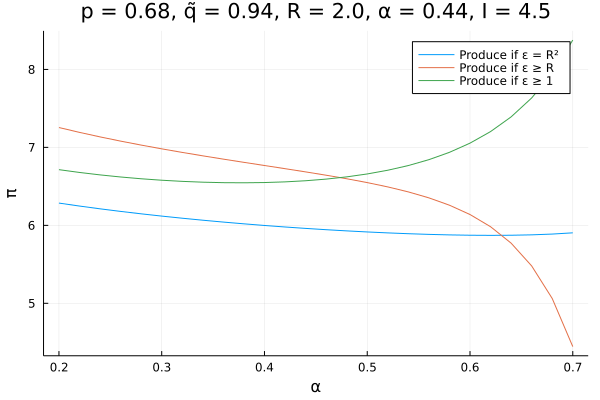
\includegraphics[scale = 0.5]{plot_alpha.png}

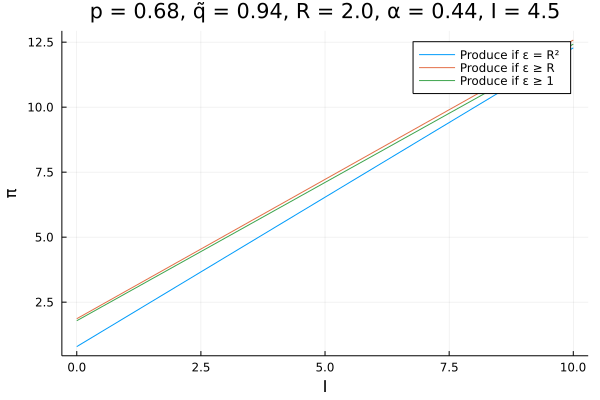
\includegraphics[scale = 0.5]{plot_I.png}

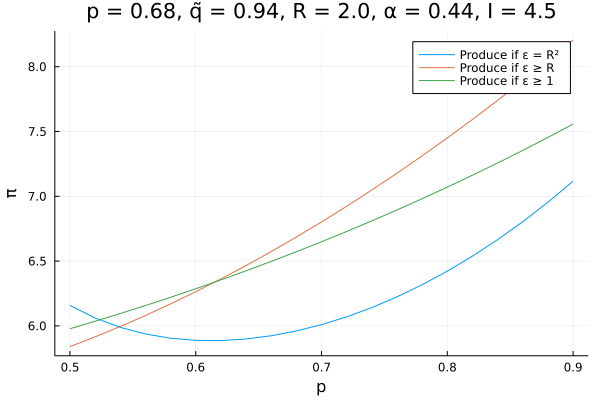
\includegraphics[scale = 0.5]{plot_p.png}

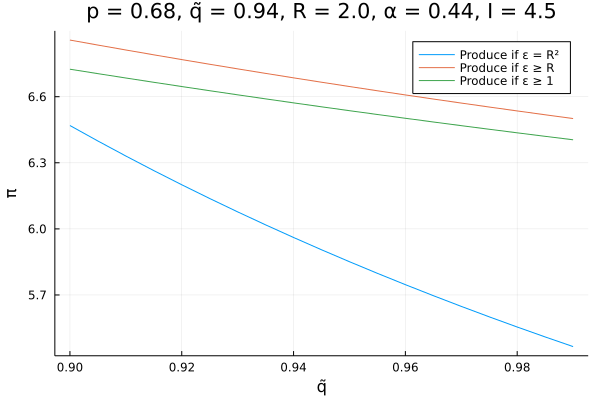
\includegraphics[scale = 0.5]{plot_q_tilde.png}

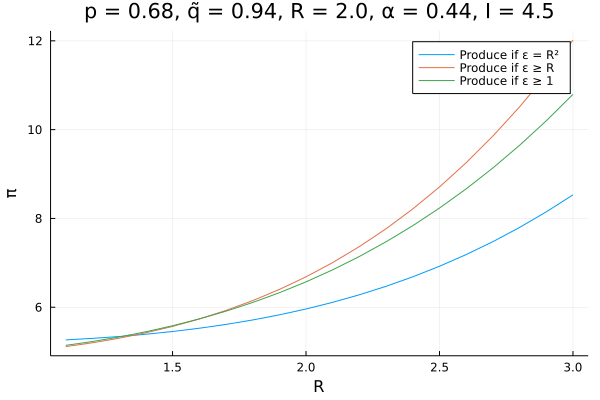
\includegraphics[scale = 0.5]{plot_R.png}

\end{center}

\pagebreak

\section*{Uniform productivity shocks}

\textbf{Simplifying assumptions:}

\begin{itemize}
\item In period 2, firm can only choose to produce or default (no reorganizing)
\item Recovery value is zero: $\xi = 1$
\item $\varepsilon_1$ and $\varepsilon_2$ are iid $U(0,1/2)$
\item One type of debt: $b_1 = 0$
\item Production function $f(\varepsilon_1,\varepsilon_2, k) = (\varepsilon_1+\varepsilon_2)k^\alpha$ for $\alpha \in (0,1)$
\end{itemize}

With these assumptions, problem is equivalent to two period model with one productivity shock $\tilde \varepsilon \sim U(0,1)$

\smallskip

\textbf{Timing with simplifying assumptions:}

\begin{itemize}
\item Period 0
\begin{itemize}
\item Firm is born with funds $I$
\item Firm sells $b$ discount bonds at price $q$ to representative risk-neutral investor who can also buy risk-free discount bonds with price $\tilde q$
\item Firm buys capital $k \equiv I + q b$ 
\end{itemize}
\item Period 1
\begin{itemize}
\item Productivity shock $\tilde \varepsilon \sim U(0,1)$ realized
\item Firm chooses to produce or default
\begin{itemize}
\item If firm produces, firm payoff is $\tilde \varepsilon k^\alpha - b$, and investor payoff is $b$
\item If firm defaults, firm payoff is 0, investor's payoff is 0
\end{itemize}
\end{itemize}
\end{itemize}

\textbf{Solution:}

\begin{itemize}

\item In period 1, firm produces iff $\tilde \varepsilon k^\alpha - b \ge 0 \implies \tilde \varepsilon \ge \frac{b}{k^\alpha}$. Notice that this threshold is increasing in $b$ and decreasing in $k$. That is if the firm has more debt (or less capital), it defaults for a larger measure of productivity shocks.

\item Thus, the firm's profit is

\begin{align*}
\pi(\tilde \varepsilon, k, b) = \begin{cases} \tilde \varepsilon k^\alpha - b, & \text{if }  \frac{b}{k^\alpha} \le \tilde\varepsilon \le 1 \\ 0, & \text{if } 0 \le \tilde\varepsilon < \frac{b}{k^\alpha} \end{cases}
\end{align*}

\item Thus, the firm's expected profit is

\begin{align*}
\pi(k,b) 
&= \int_0^1 \pi(\tilde \varepsilon, k, b) d \tilde \varepsilon\\
&= \int_{0}^{b/k^\alpha}  \pi(\tilde \varepsilon, k, b) d \tilde \varepsilon  + \int_{b/k^\alpha}^1 \pi(\tilde \varepsilon, k, b) d \tilde \varepsilon \\  &= 0+\int_{b/k^\alpha}^1 (\tilde \varepsilon k^\alpha - b) d \tilde \varepsilon \\
&= \Bigg[\frac{1}{2}\tilde \varepsilon^2 k^\alpha -\tilde \varepsilon b \Bigg]_{b/k^\alpha}^1\\
&= \frac{1}{2} k^\alpha - b - \frac{1}{2}(b/k^\alpha)^2 k^\alpha + (b/k^\alpha) b\\
&= \frac{1}{2} k^\alpha - b - \frac{1}{2}b^2 k^{-\alpha} + b^2 k^{-\alpha}\\
&= \frac{1}{2} k^\alpha - b + \frac{1}{2}b^2 k^{-\alpha}
\end{align*}

The first term is the expected output conditional on the firm producing, the second term is the (expected) debt repayment again conditional on the firm producing, and the third term is a positive term that accounts for the option value of defaulting. This term is increasing in debt $b$ and decreasing in capital $k$ because the measure of productivity shocks for which the firm defaults grows with more debt or less capital. So the option to default is more valuable.

\item In period 0, taking $q$ as given, firm chooses $k$ and $b$ to maximize expected profit in period 1:

\begin{align*}
\max_{k,b} & \;\;\pi(k,b) \\ 
\text{s.t. } & k = I + bq \\
\implies
\Lfn &= \frac{1}{2} k^\alpha - b + \frac{1}{2}b^2 k^{-\alpha} + \lambda (I + bq - k)
\end{align*}

\item FOCs

\begin{align*}
\frac{\alpha}{2} k^{\alpha-1} &= \frac{\alpha}{2}b^2 k^{-\alpha-1} + \lambda & [k] \\
 b k^{-\alpha} + \lambda q &= 1 & [b] \\
\end{align*}

$\lambda$ can be interpreted as the value of relaxing the feasibility constraint that capital equals internal funds plus proceeds from the sale of discount bonds.  Thus, the choice of $k$ equates the marginal product of capital (marginal benefit of higher $k$; LHS) to the marginal decrease in the option value of defaulting plus the value of the feasibility constraint (marginal cost of higher $k$; RHS). And the choice of $b$ equates the increase in the option value of default plus the value of loosening the feasibility constraint (marginal benefit of higher $b$; LHS) to one (the marginal cost of higher $b$; RHS)

\item Combining FOCs:

\begin{align*}
 b k^{-\alpha} + q\frac{\alpha}{2} k^{\alpha-1} &= 1 + q\frac{\alpha}{2}b^2 k^{-\alpha-1} 
\end{align*}

\item The lender's zero profit condition pins down $q$.  The risk-neutral lender buy risk-free bonds that is invest $\tilde q b$ and get $b$ for certain. Or she can buy risky bonds that is invest $q b$ and get get $b$ with probability if the firm produces.

\begin{align*}
\int_0^1b d\tilde \varepsilon - \tilde q b &= \int_{b/k^\alpha}^1 b d \tilde \varepsilon - qb \\ 
\implies
b - \tilde q b &= b (1-b/k^\alpha) - qb \\ 
\implies
1 - \tilde q &= 1-b/k^\alpha - q\\ 
\implies
q &= \tilde q - b/k^\alpha
\end{align*}

Thus, $q < \tilde q$. A lower discount bond price corresponds to a higher interest rate; the risky bonds pay premium over risk-free rate.  The premium over the risk-free rate increases in $b$ and decreases in $k$.


\item Substitute in lender's zero profit condition into firm FOC and feasibility constraint

\begin{align*}
b k^{-\alpha} + (\tilde q - b/k^\alpha)\frac{\alpha}{2} k^{\alpha-1} &= 1 + (\tilde q - b/k^\alpha)\frac{\alpha}{2}b^2 k^{-\alpha-1} \\
 k &= I + b(\tilde q - b/k^\alpha)
\end{align*}

to get two nonlinear equations in two unknowns $(k, b)$

\pagebreak

\item Allow $b_1 \neq 0$

\item Timing

\begin{itemize}
\item Period 0
\begin{itemize}
\item Firm is born with funds $I$
\item Firm sells $b_0$ discount bonds at price $q_0$ to representative risk-neutral ``long-term" investor who can also buy risk-free discount bonds with price $\tilde q$
\end{itemize}
\item Period 1
\begin{itemize}
\item First productivity shock $\varepsilon_1 \sim U(0,1/2)$ realized
\item Firm sells $b_1$ discount bonds at price $q_1$ to representative risk-neutral ``short-term" investor who can also buy risk-free discount bonds with price $\tilde q$
\item Firm buys capital $k \equiv I + q_0 b_0 + q_1 b_1$ and has outstanding debt $b \equiv b_0 + b_1$
\end{itemize}
\item Period 2
\begin{itemize}
\item Second productivity shock $\varepsilon_2 \sim U(0,1/2)$ realized
\item Firm chooses to produce or default
\begin{itemize}
\item If firm produces, firm payoff is $f(\varepsilon_1, \varepsilon_2, k) - b$, long-term investor payoff is $b_0$, and long-term investor payoff is $b_1$
\item If firm defaults, firm payoff is 0, long-term investor's payoff is $0$, short-term investor's payoff is $0$ 
\end{itemize}
\end{itemize}
\end{itemize}

\item In period 2, firm produces iff $(\varepsilon_1 + \varepsilon_2) k ^ \alpha - b_0 - b_1 \ge 0 \implies \varepsilon_2 \ge \frac{b_0 + b_1}{k^\alpha} - \varepsilon_1$

\item Firm profit is

\begin{align*}
\pi(\varepsilon_1, \varepsilon_2, k, b_0+b_1) = \begin{cases} (\varepsilon_1 + \varepsilon_2) k^\alpha - b_0 - b_1, & \text{if }  \frac{b_0 + b_1}{k^\alpha} - \varepsilon_1 \le \varepsilon_2 \le 1 \\ 0, & \text{if } 0 \le \varepsilon_2 < \frac{b_0 + b_1}{k^\alpha} - \varepsilon_1 \end{cases}
\end{align*}

\item Thus, the firm's expected profit is

\begin{align*}
\pi(k,b) 
&= \int_0^1 \pi(\tilde \varepsilon, k, b) d \tilde \varepsilon\\
&= \int_{0}^{b/k^\alpha}  \pi(\tilde \varepsilon, k, b) d \tilde \varepsilon  + \int_{b/k^\alpha}^1 \pi(\tilde \varepsilon, k, b) d \tilde \varepsilon \\  &= 0+\int_{b/k^\alpha}^1 (\tilde \varepsilon k^\alpha - b) d \tilde \varepsilon \\
&= \Bigg[\frac{1}{2}\tilde \varepsilon^2 k^\alpha -\tilde \varepsilon b \Bigg]_{b/k^\alpha}^1\\
&= \frac{1}{2} k^\alpha - b - \frac{1}{2}(b/k^\alpha)^2 k^\alpha + (b/k^\alpha) b\\
&= \frac{1}{2} k^\alpha - b - \frac{1}{2}b^2 k^{-\alpha} + b^2 k^{-\alpha}\\
&= \frac{1}{2} k^\alpha - b + \frac{1}{2}b^2 k^{-\alpha}
\end{align*}

\end{itemize}

\end{document}




